\chapter{Разработка и реализация методов эффективного взаимодействия процессов}
\textbf{TBD: починить - в листингах}
%
%\section{Интерфейс доступа к разрабатываемым методам межпроцессного взаимодействия}
%
%\textbf{TBD: можно взять из бакалаврской ВКР или оставить на нее ссылку.}
%
%Существенная часть межпроцессного взаимодействия - это то, как программист его использует и как сделать это удобным процессом. Интерфейс сокетов в ОС Linux хорошо для этого, так как использует механизм файловых дескрипторов
%\textbf{TBD: определение или ссылку}
%, а значит:
%\begin{itemize}
%\item имеет стандартные примитивы чтения и записи: системные вызовы \textit{read/readv} и \textit{write/writev};
%\item позволяет мультиплексировать множество соединений для одновременного отслеживания посредством системных мультиплексоров: \textit{select/poll/epoll}.
%\end{itemize}
%
%Удобный и унифицированный интерфейс может объединять под собой совершенно разные методы межпроцессного взаимодействия прозрачным для программиста образом. Программист зачастую не заинтересован в тонкостях передачи данных, ему необходимо реализовывать и совершенствовать пользовательскую логику приложения, однако, поскольку процессы распределенной системы работают вместе над одними задачами, то ему важна и эффективность межпроцессного взаимодействия.
%
%Необходима возможность:
%\begin{itemize}
%\item предоставлять другим процессам возможность для подключения и подключаться к другим процессам;
%\item принимать и передавать данные.
%\end{itemize}
%
%Для первого пункта хорошо подходит семейство шаблонов сетевого программирования Acceptor и Connector \cite{schmidt1996acceptor}, которые при необходимости создают экземпляры пользовательских обработчиков соединений, реализующих интерфейс, представленный на листинге \ref{chapter31:ServiceHandlerInterface}.
%
%\begin{lstlisting}[float=!h,caption={Интерфейс пользовательского обработчика соединений на C++},label={chapter31:ServiceHandlerInterface}]
%class ISession
%{
%public:
%	virtual int handle_message(const Message & message) = 0;
%	virtual int send(const Message & message) = 0;
%	virtual int handle_close() = 0;
%};
%\end{lstlisting}
%
%%Поскольку существует необходимость полностью оградить программиста от тонкостей работы межпроцессного взаимодействия, чтобы упростить работу пользовательского кода и иметь возможность выбирать наиболее подходящий для данной ситуации метод межпроцессного взаимодействия. выбран событийный асинхронный метод доставки сообщений. Для этого в интерфейсе пользовательского обработчика соединения предусмотрен метод \textit{handle\_message(const Message \&)}. Нижележащая реализация метода межпроцессного взаимодействия вызывает данный метод для соответствующего соединения по факту получения ей очередного сообщения. Для отправки сообщений программисту предлагается использовать примитив \textit{send(const Message \&)}.
%
%\textbf{TBD: кривовато звучит}
%Данный интерфейс соответствует асинхронному событийному шаблону проектирования приложений. В этом шаблоне обработчик соединения является пассивной сущностью, в которую события доставляются посредством вызова метода \textit{handle\_message(const Message \&)}. Во-первых, использование этого шаблона позволяет разделить пользовательскую логику и нижележащие методы межпроцессного взаимодействия, работающие по произвольным алгоритмам. Следовательно, это упрощает пользовательскую логику. Во-вторых, позволяет обрабатывать множество соединений числом потоков, не равным количеству этих соединений, так как обработчики соединения нуждаются в потоке для своего выполнения только когда необходимо обработать событие. Для отправки сообщений программисту предлагается использовать примитив \textit{send(const Message \&)}.
%
%Данный интерфейс позволяет скрыть от программиста тонкости работы межпроцессного взаимодействия. Например, отслеживание готовности множества TCP-соединений к передаче или приему данных, состояние соединений. Или то, что взаимодействие происходит через разделяемую память.
%
%\section{Базовый метод межпроцессного взаимодействия на основе TCP}\label{chapter31:PureTCP}
%
%TCP -- это наиболее широко-используемый и универсальный метод межпроцессного взаимодействия. Протокол гарантирует, что сообщения будут получены в том же количестве и порядке, в котором они были отправлены. Посредством интерфейса сокетов он позволяет взаимодействовать как с локальными, так и с удаленными процессами распределенной системы. Более того, сторонние системы тоже зачастую предоставляют возможность именно подключения по TCP.
%
%Кроме распространенности и удобства для программиста, предоставляют очень важную возможность отслеживания времени жизни соединения. Это важно, так как случае краха процесса операционная система в ходе освобождения системных ресурсов также закроет все TCP-соединения процесса и другие стороны межпроцессного взаимодействия смогут корректно обработать закрытие соединений.
%
%\subsection{Мультиплексирование соединений}
%
%Межпроцессное взаимодействие посредством TCP позволяет использовать системные мультиплексоры оповещений \textit{select/poll/epoll} для отслеживания оповещений в множестве TCP-соединений: наличия данных, готовности канала к передаче, закрытия соединения. В системах с большим количеством неактивных соединений лучше всего себя показывает системный мультиплексор \textit{epoll}, при наличии небольшого количества активных соединений большой разницы между ними не наблюдается \cite{MuxComparison}.
%
%Классическим подходом при разработке сетевых приложений является применение шаблона Реактор \cite{schmidt1995reactor, 10.1145/1808954.1808964} для диспетчеризации множества соединений. В настоящей работе используется реализаций шаблона Реактор из библиотеке ACE \cite{ACE}, работающая с системным мультиплексором оповещений \textit{select}.
%
%Реактор -- это объект, в котором регистрируются обработчики событий и которые Реактор вызывает посредством вызовов их интерфейсных методов. Сокращенный интерфейс обработчика событий из библиотеки ACE приведен в листинге \ref{chapter31:LowLevelServiceHandlerInterface}.
%\begin{lstlisting}[float=!h,caption={Интерфейс низкоуровневого обработчика соединений на C++},label={chapter31:LowLevelServiceHandlerInterface}]
%class ACE_Event_Handler
%{
%public:
%	virtual int handle_input(ACE_HANDLE fd) = 0;
%	virtual int handle_output(ACE_HANDLE fd) = 0;
%	virtual int handle_close(ACE_Handle fd, ACE_Reactor_Mask close_mask) = 0;
%};
%\end{lstlisting}
%
%\textbf{TBD}
%
%\subsection{Обслуживание активных соединений}
%
%\textbf{TBD}
%
%\subsection{Динамическое конфигурирование соединений}
%\textbf{TBD: надо написать про стек модулей}
%
%
%\section{Применение разделяемой памяти для передачи данных}
%
%\textbf{TBD: описать SPSC очередь на буфере постоянного размера}
%
%Однако, недостаточно разместить очередь в разделяемой памяти и отправлять в нее сообщения. Кроме контроля времени жизни соединения, существенный вопрос в данном методе: кто, как и когда будет принимать сообщения. На одном физическом узле может находится множество взаимодействующих процессов с большим количеством соединений между ними. Соответственно, для каждого соединения появляется своя точка синхронизации, в которой процесс-читатель может узнать, что очередь не пуста.
%
%Необходимо разработать метод оповещения процесса-читателя о появлении данных в разделяемой памяти, которые ему необходимо принять и обработать.

\section{Работа с очередью в разделяемой памяти}\label{chapter31:SharedMemoryOptimization}

\textbf{TBD: module stack, handshake}
\textbf{TBD: нужна иллюстрация взаимодействия или какой- нибудь псевдокод}

\section{Методы оповещения о появлении данных в разделяемой памяти}

\subsection{Наивные алгоритмы в разделяемой памяти}

Процесс-читатель знает о расположении всех очередей в разделяемой памяти, в которые отправляют сообщения все процессы-писатели, с которыми он взаимодействует. Непосредственно само состояние очередей может быть использовано для оповещения процесса-читателя о появлении данных в этих очередях.

\paragraph{Алгоритм №1}

При небольшом количестве соединений (например, $0.25 * N$, где $N$ - количество ядер в процессоре) возможно использование выделенных потоков в процессе-читателе для активного опроса состояния очереди и обслуживания соответствующего соединения.  \textbf{TBD: иллюстрацию?}

\paragraph{Алгоритм №2}

При большем количестве соединений возможно использовать группу выделенных потоков, активно опрашивающих которое количество очередей в разделяемой памяти. Например, 1 поток, активно опрашивающий до 10 соединений.
\textbf{TBD: иллюстрацию?}

\subsubsection{Применимость, достоинства и недостатки}\label{chapter31:NaivePolling}

Данные алгоритмы активного опроса очередей в разделяемой памяти для обслуживания соединений вполне могут быть использованы в реальных системах. Их можно применить в системах: с большими вычислительными ресурсами, небольшим количеством процессов и очень активных соединений.

В противном случае, активно работающие потоки будут выполнять много бесполезных операций по опросу пустых очередей неактивных соединений. Кроме того, постоянно работающий поток, опрашивающий очереди в разделяемой памяти, может быть вытеснен с процессора планировщиком операционной системы из-за израсходования отведенного ему кванта процессорного времени, что ухудшит качество обслуживания заявок.

Приведенные методы в настоящей работе не рассматриваются, поскольку количество соединений между процессами на одном физическом узле и самих процессов может быть большим, а опрос очередей на наличие в них данных сопровождается взятием взаимной блокировки, что приводит к неэффективному использованию аппаратных ресурсов.

\subsection{TCP}\label{chapter31:SignalTCP}

Как было сказано выше, TCP используется как базовый метод межпроцессного взаимодействия. Он может быть использован и как метод оповещения о появлении данных в очереди в разделяемой памяти.

\subsubsection{Алгоритм взаимодействия при использовании TCP для оповещения о появлении данных}

\textbf{TBD: нужна иллюстрация взаимодействия и стек модулей}
% Чтобы процесс-читатель о наличии данных в очереди в разделяемой памяти, необходимо:

\begin{enumerate}
\item процессу-читатель ожидает новых данных по всем своим TCP соединениям в состоянии сна в системном мультиплексоре оповещений;
\item для передачи данных таким методом процессу-писателю необходимо записать в очередь нужное сообщение и передать на нижележащий модуль сообщение минимального размера в 1 байт с заранее установленным значением (например, ''0``);
\item ядро операционной системы пробуждает процесс-читатель;
\item реактор процесса-читателя демультиплексирует активное TCP соединение, считывает 1 байт полезных данных и отправляет его на следующий слой обработки межпроцессных взаимодействий через ранее описанный стек модулей;
\item модуль, отвечающий за взаимодействие по разделяемой памяти, проверяет, что полученный 1 байт имеет заранее оговоренное значение (''0`` в примере выше) и это служит для него сигналом к проверке состояния очереди в разделяемой памяти для соединения, с которого этот сигнальный байт был получен;
\item процесс-читатель считывает сообщение из очереди и выполняет его обработку.
\end{enumerate}

Таким образом происходит передача данных между процессами в разделяемой памяти с оповещением о появлении данных в разделяемой памяти по TCP.

\subsubsection{Достоинства и недостатки}

Предложенный метод обладает следующими \textbf{достоинствами}:
\begin{itemize}
\item позволяет эффективно поддерживать множество соединений с использованием системных мультиплексоров оповещений (\textit{select/poll/epoll});
\item позволяет процессу-читателю блокировать свое выполнение до появления оповещения;
\item благодаря использованию эвристики из раздела \ref{chapter31:SharedMemoryOptimization} временная задержка на передачу данных может быть снижена, если к концу обработки очередного сообщения в очередь уже будет записано новое сообщение;
\item метод межпроцессного взаимодействия по TCP не требует доработки и может быть использован как есть.
\end{itemize}

\textbf{Недостаток} у такого подхода только один: временная задержка на отправку и получение оповещения. Основные отличия от метода, использующего только TCP, в том, как передается само сообщения. Но кроме использования среды для передачи самих данных выполняется рад системных вызовов для оповещения процесса-читателя, каждый из которых может вносить существенную временную задержку:
\begin{itemize}
\item \textit{write} -- для записи 1 байта в TCP-сокет процессом-писателем;
\item \textit{select/poll/epoll} -- для демультиплексирования нужного оповещения среди множества источников процессом-читателем.
\item \textit{read} -- для чтения 1 байта из TCP-сокета процессом-читателем.
\end{itemize}

В случае, когда процесс-читатель находится в состоянии сна на системном мультиплексоре оповещений, процесс-писатель в ходе системного вызова \textit{write} должен также изменить состояние процесса-читателя на ''Готов к выполнению`` или ''Выполняется``. После этого в течение некоторого промежутка времени процесс-читатель будет готовиться к выполнению. Все это может влиять на временную задержку на передачу данных.

Следовательно, необходимо разработать новый метод мультиплексирования соединений, использующих разделяемую память, имеющий меньшие накладные расходы на использование и обладающий, как минимум, теми же достоинствами, что и описанный в данном разделе. 

\subsection{Мультиплексор оповещений в разделяемой памяти}\label{chapter31:Mux}

С целью избежать излишних накладных расходов и использовать системные ресурсы наилучшим образом в настоящей работе предлагается метод мультиплексирования оповещений от множества соединений, использующих разделяемую память для передачи данных.

Мультиплексор оповещений в разделяемой памяти -- это структура данных, используемая множеством процессов-писателей для оповещения процесса-читателя о появлении данных в очереди в разделяемой памяти. Каждый процесс, участвующий в межпроцессном взаимодействии, должен иметь свой мультиплексор оповещений, через который ему будут поступать оповещения о появлении данных в разделяемой памяти, которые он может считать и обработать.

Время жизни мультиплексора оповещений определяется процессом-читателем. При необходимости процесс-читатель создает файл определенного размера в ФС и отображает его в свою память. Во время установления соединения процесс-читатель ассоциирует соединение с номером от 0 до 2047 и отправляет его вместе с путем до файла другой стороне. Эти данные используются противоположной стороной для отправки оповещений.

\textbf{TBD: нарисовать схему с двумя процессами и файлом, отображенным в их памяти}

\subsubsection{Структура и алгоритм работы мультиплексора оповещений в разделяемой памяти}\label{chapter31:MuxStructure}

Структура мультиплексора оповещений представлена на рисунке \ref{chapter31:MuxZeroState}. Он состоит из 4-байтного целого числа futex, используемого для синхронизации взаимодействующих процессов, и массив из 32 8-байтных сигнальных чисел, по одному на каждый бит futex. Эти 32 8-байтных числа содержат 2048 бит, что позволяет различать 2048 различных соединений. Описание на языке C++ представлено на листинге \ref{chapter31:MultiplexerStruct}.


\begin{figure}[!h]
\caption{Структура мультиплексора оповещений в разделяемой памяти}
\label{chapter31:MuxZeroState}
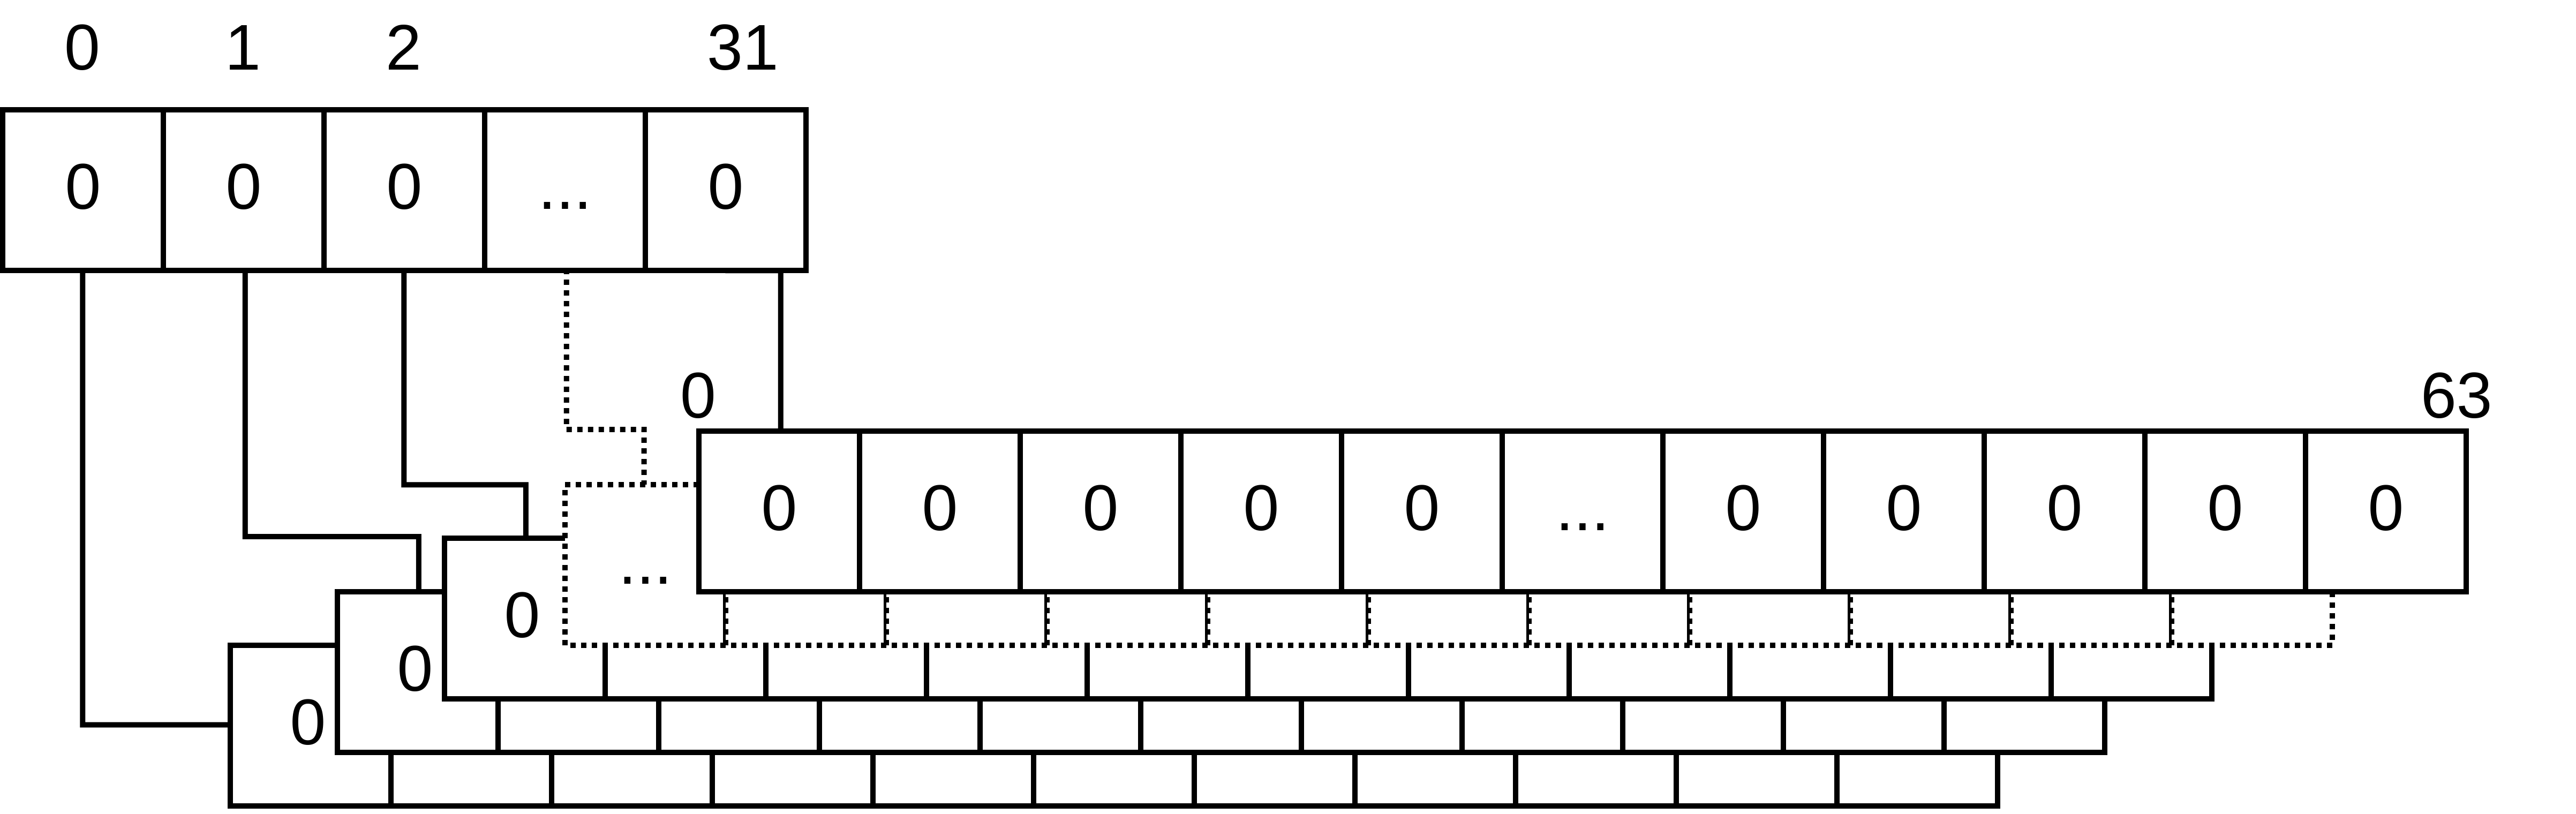
\includegraphics[width=\textwidth]{../../graphics/schemes/futex}
\end{figure}

\begin{lstlisting}[float=!h,caption={Структура мультиплексора в памяти},label={chapter31:MultiplexerStruct},frame=tlrb]
struct Multiplexer
{
    using Futex = std::atomic<int32_t>;
    using Signal = uint64_t;

    static constexpr std::size_t c_num_chunks = sizeof(Futex) * CHAR_BIT;
    static constexpr std::size_t c_signals_per_chunk = sizeof(std::atomic<Signal>) * CHAR_BIT;
	
	// Процедура ожидания на futex
    void wait() {
    	if (!m_futex) {
   			futex_wait(&m_futex, 0);
   		}
    }
	
	// Процедура оповещения процесса--читателя. Выставляет соответствующие биты мультиплексора для сигнала за номером signal и при необходимости пробуждает поток мультиплексора процесса-читателя.
    void notify(Multiplexer::Signal id);
    
    // Процедура для пробуждения потока, спящего на futex.
    void wakeup();

protected:
	// 4--байтное число futex, на котором происходит синхронизация сна/пробуждения потока мультиплексора.
    Futex m_futex;
	
	// Для избежания лишней состязательности между атомарными операциями над массивом сигнальных чисел и над futex, массив выровнен на размер кэш-линии процессора -- 64 байта.
    alignas(64) std::array<std::atomic<Signal>, c_num_chunks> m_signals;
};
\end{lstlisting}

Когда процесс-писатель хочет оповестить процесс-читатель о появлении данных в очереди в разделяемой памяти, ему необходимо:
\begin{enumerate}
\item атомарно выставить бит в сигнальном числе, соответствующий этому соединению;
\item атомарно выставить соответствующий бит futex и получить его предыдущее значение;
\item Если предыдущее значение равно нулю, значит, разбудить процесс-читатель, чтобы он мог обработать оповещение.
\item Если оно не равно нулю, это значит, что другой процесс-писатель уже либо разбудил целевой процесс-читатель, либо в скором времени сделает это (так как он был тем самым процессом, перед которым в futex был нуль).
\end{enumerate}

После завершения первых двух этапов мультиплексор для соединения под номером \#1987 будет находиться в состоянии, представленном на рисунке \ref{chapter31:Mux1987State}. Чтобы проставить нужные биты для данного, процесс-писатель делит номер его соединения на 64 и получает индекс бита в futex -- 31, и, соответственно, индекс сигнального числа. Далее он вычисляет остаток от деления номера сигнала на 64 и получает индекс бита в сигнальном числе. После чего атомарной операцией ''ИЛИ`` выставляется сначала нужный бит в сигнальном числе, а потом нужный бит в futex. Псевдокод алгоритмов процесса-писателя и читателя приведены на листингах \ref{chapter31:SignalCode} и \ref{appendix91:ReceiverCode}.

\begin{algorithm}[!h]
\caption{Исходный код процедуры оповещения процесса через мультиплексор событий в разделяемой памяти}
\label{chapter31:SignalCode}
\begin{lstlisting}[frame=tlrb]
void Multiplexer::notify(Signal id) {
	// Шаг 1. Выставить нужный бит в одном из сигнальных чисел в массиве. Число находится как результат деления номера соединения на 64, т.е. число от 0 до 31, позиция бита как остаток от деления номера соединения на 64.
	m_signal[id / Multiplexer::c_signals_per_chunk].fetch_or(1 << id % Multiplexer::c_signals_per_chunk);
    // Шаг 2. Выставить бит futex, соответствующий сигнальному числу. Позиция нужного бита находится как результат деления нмоера соединения на 64, т.е. число от 0 до 31.
	uint32_t futex = m_futex.fetch_or(1 << id / Multiplexer::c_signals_per_chunk);
	if (!futex) {
		// Шаг 3. Если предыдущее значение futex было 0, то попытаться разбудить один процесс, спящий на futex, системным вызовом futex.
		this->wakeup();
	}
}
\end{lstlisting}
\end{algorithm}

\begin{figure}[!h]
\caption{Состояние мультиплексора оповещений в разделяемой памяти с активным сигналом \#1987}
\label{chapter31:Mux1987State}
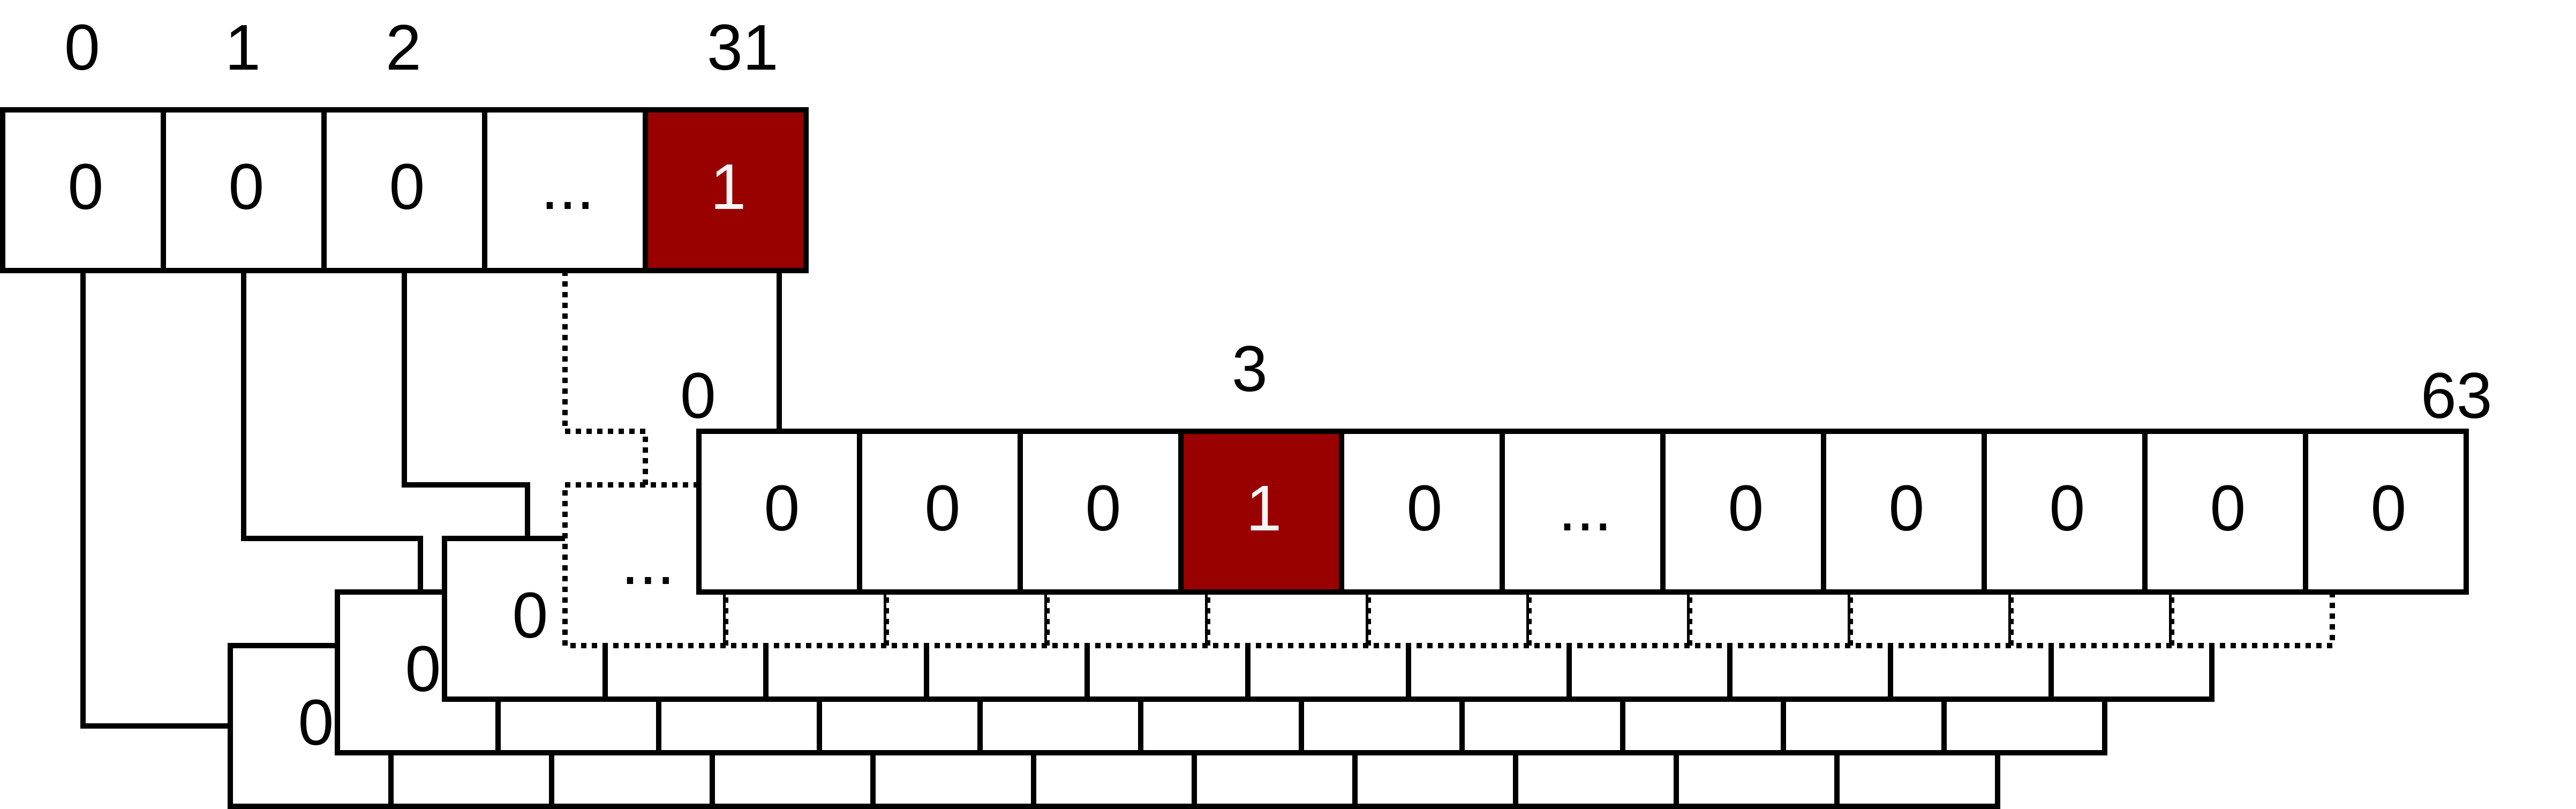
\includegraphics[width=\textwidth]{../../graphics/schemes/futexready}
\end{figure}

\subsubsection{Достоинства и недостатки}

Данный метод решает проблему, описанную в разделе \ref{chapter31:NaivePolling}, позволяя определять соединение-источник сигнала за время, не зависящее от количества соединений.

По сравнению с вышеописанным методом межпроцессного взаимодействия, использующим TCP для оповещения о появлении данных в разделяемой памяти, данное решение обладает следующими \textbf{достоинствами}:
\begin{enumerate}
\item Подавляющая часть работы происходит в пользовательском пространстве. В лучшем сценарии отправка и получение оповещения не задействуют системные вызовы. Оповещение происходит посредством двух атомарных операций.
\item Ядро ОС используется только пробуждения и засыпания процессов.
\end{enumerate}

Таким образом, в худшем случае совершается один системный вызов для засыпания процесса в ожидании оповещений и один для пробуждения процесса. Пробуждение потока влечет временные затраты как со стороны процесса-писателя -- на пробуждение потока, так и со стороны процесса-читателя -- на уход в состояние сна и временную задержку на постановку потока мультиплексора на выполнение. В то же время, ожидание оповещений в состоянии сна позволяет экономить ресурс процессора.

\textbf{Недостатком} данного метода является механизм управление файлом мультиплексора оповещений в файловой системе. Поскольку файлом управляет процесс, то в случае его некорректного завершения файл не будет удален и останется на всегда. Некорректное завершение может произойти по следующим причинам: крах процесса вследствие программного дефекта, при отправке сигнала \textit{SIGKILL} процессу, который в большинстве случаев приводит к немедленному завершению процесса.

Данный недостаток можно решить, используя более продвинутый механизм создания файлов в ФС. Например, делегировать эту работу отдельному процессу или группе процессов. В таком случае такой процесс может отслеживать состояние своих клиентских процессов и при прекращении их работы выполнять подчистку ресурсов.

\subsection{Методы обслуживания соединений}

Имея более совершенный механизм оповещения процессов о появлении данных в разделяемой памяти необходимо разработать также и метод обслуживания получаемых оповещений. В данном подразделе предложены четыре метода:
\begin{enumerate}
\item Синхронный -- существует единственный выделенный поток мультиплексора. Он занимается непосредственно обслуживанием соединений.
\item ''Полусинхронный/Полуреактивный`` -- существует единственный выделенный поток мультиплексора (полуреактивная часть). Он диспетчеризует обслуживание оповещений в пул потоков (полусинхронная часть) \cite{schmidt1995half}.
\item ''Лидер/Последователи`` -- в один момент времени только один поток-лидер отслеживает состояние мультиплексора в пассивном режиме. То есть, при отсутствии оповещений процесс-лидер находится в состоянии сна. При обнаружении оповещений он передает лидерство произвольному потоку из пула и переходит к обслуживанию оповещений \cite{schmidt1998leader}.
\item ''Лидер/Последователи`` -- в один момент времени только один поток-лидер активно отслеживает состояние мультиплексора. То есть, постоянно опрашивает мультиплексор. При обнаружении оповещений он передает лидерство произвольному потоку из пула и переходит к обслуживанию оповещений.
\end{enumerate}

\subsubsection{Синхронный метод обслуживания соединений}

В данном методе для обслуживания оповещений выделяется один поток, который обслуживает только соединения, использующие мультиплексор оповещений. Диграмма его работы представлена на рисунке \ref{chapter31:SyncMuxSchema}.
В отсутствие заявок поток мультиплексора находится в состоянии сна. Когда необходимо обработать соединение, ядро пробуждает этот поток и он, в свою очередь, выполняет алгоритм на листинге \ref{appendix91:ReceiverCode}, синхронно обрабатывая соединения, для которых были получены оповещения. Алгоритм выполняется до тех пор, пока есть оповещения для обслуживания.

Метод может быть полезен для систем с малым количеством соединений. Из-за своей простоты он может показать лучшую временную задержку на передачу данных, так как нет необходимости, как в других методах, диспетчеризовать обслуживание соединения в пуле потоков или выбирать новый поток-лидер перед обслуживанием данного соединения.

Однако, поскольку поток, обслуживающий мультиплексор, один, то когда он обслуживает текущее соединение, все остальные активные соединения простаивают. Данный метод далее в работе не рассматривается, так как не смотря на потенциально более низкую временную задержку на передачу данных при его использовании, он ограничен в количестве одновременно активных соединений.

\begin{figure}[!h]
\caption{Диаграмма синхронного обслуживания соединений выделенным потоком мультиплексора}
\label{chapter31:SyncMuxSchema}
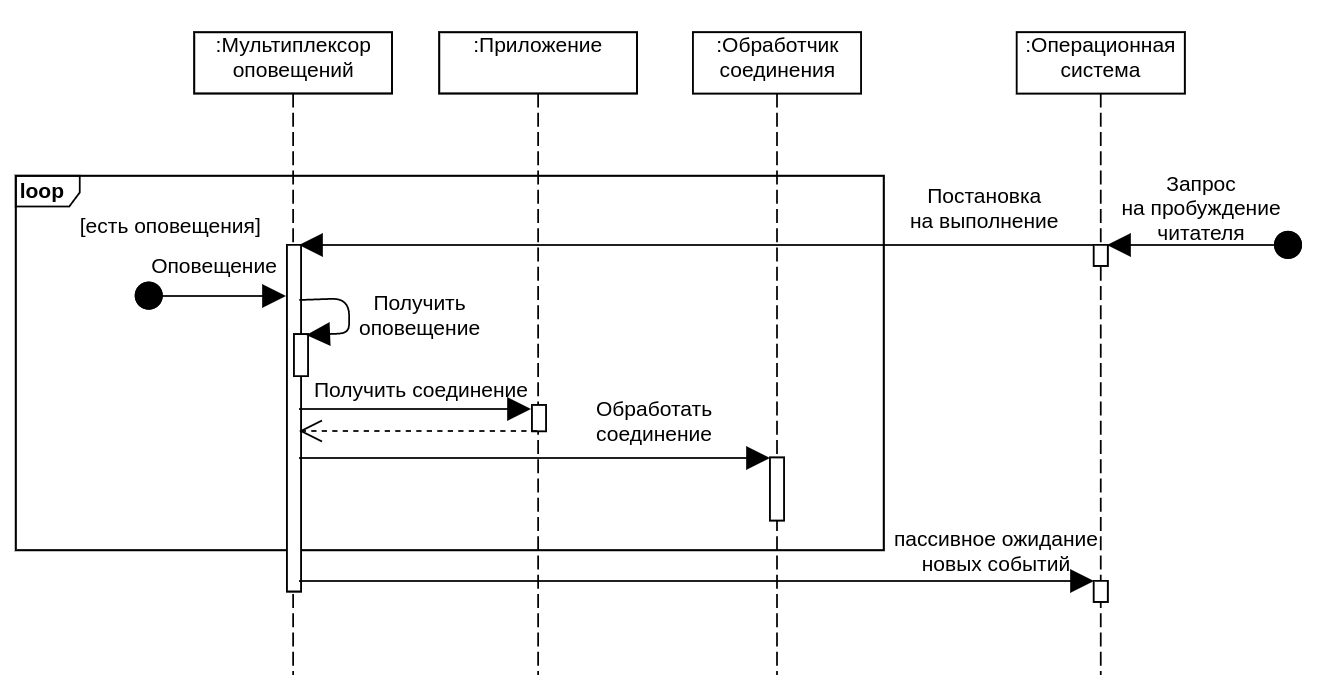
\includegraphics[width=\textwidth]{../../graphics/schemes/SyncMuxSequence}
\end{figure}


\subsubsection{Метод обслуживания соединений ''Полусинхронный/Полуреактивный``}\label{chapter31:BlockingHSHA}
Описан в ранней работе автора \cite{GubarevFutex}.
В данном методе оповещения обслуживает пул потоков. Пул потоков получает задачи на обслуживание от выделенного потока мультиплексора оповещений. Применение шаблона проектирования сетевых приложений ''Полусинхронный/Полуреактивный`` \cite{schmidt1995half} к синхронному методу позволяет избежать простаивания активных соединений и обслуживать одновременно столько же соединений, сколько потоков выделено в пуле. Диаграмма работы метода представлена на рисунке \ref{chapter31:HSHAMuxSchema}.

\begin{figure}[!h]
\caption{Диаграмма диспетчеризации и обслуживания соединений по методу ''Полусинхронный/Полуреактивный``}
\label{chapter31:HSHAMuxSchema}
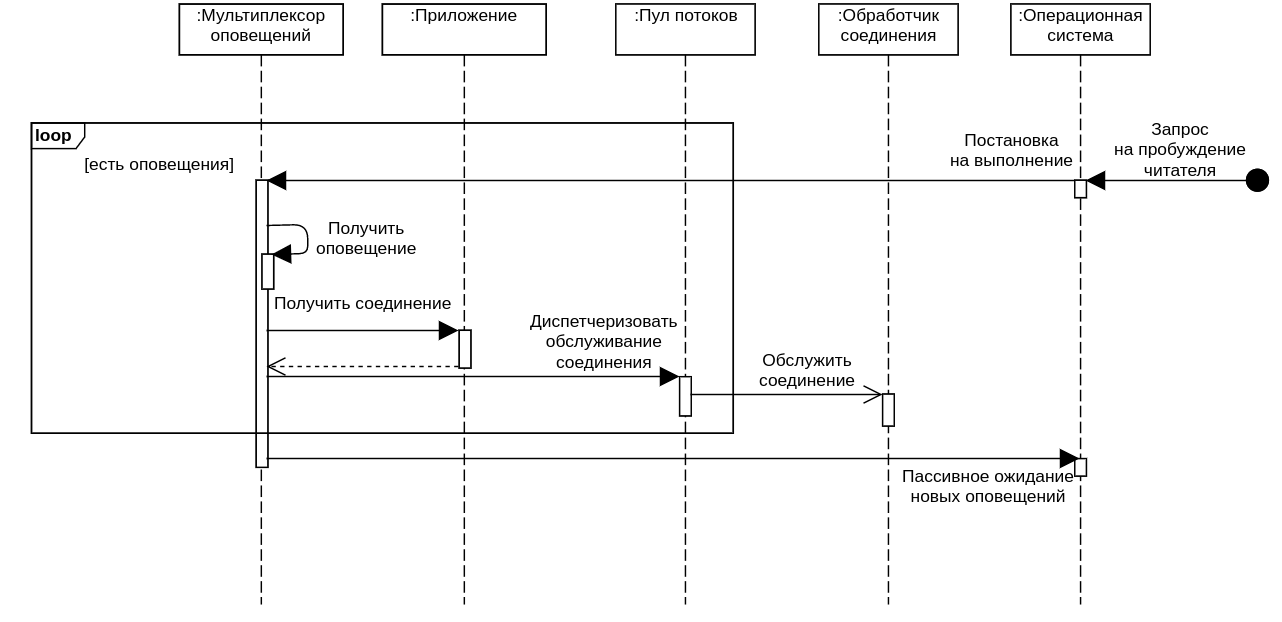
\includegraphics[width=\textwidth]{../../graphics/schemes/HSHAMuxSequence}
\end{figure}

Получение оповещений для соединения и обслуживание заявок для этого соединения происходит в разных потоках. Необходимо сохранить гарантию последовательного обслуживания заявок в соединении. То есть, в один момент времени заявки одного соединения обслуживает не более одного потока. Может произойти ситуация, при которой очередное оповещение для очередной заявки будет получено во время обслуживания текущей. В таком случае, поток из пула должен обслужить новую заявку после текущей, либо обслуживание должно быть делегировано пулу потоков после обслуживания текущей заявки. Первая стратегия предпочтительнее, так как имеет лучшую локальность по памяти и времени: один и тот же поток последовательно обслуживает заявки для одного и того же соединения при их наличии. В обоих случаях необходимо синхронизировать диспетчеризацию и непосредственно процедуру обслуживания соединения.

На листингах \ref{chapter31:DispatchHSHASession} и \ref{chapter31:ServeHSHASession} представлен исходный код процедур диспетчеризации и обслуживания соединений. Между собой процедуры синхронизированы механизмом взаимного исключения и набором состояний.

\begin{lstlisting}[float=!h,caption={Процедура диспетчеризации обслуживания соединения},label={chapter31:DispatchHSHASession},frame=tlrb]
void IMultiplexerListener::check_close_n_handle_send()
{
    std::unique_lock<std::mutex> lock(m_input_close_mutex);
    if (m_state == State::Closed) {
        return;
    }
    if (m_state == State::Handling) {
        m_state = State::KeepHandling;
        return;
    }
    m_state = State::Handling;
    lock.unlock();

    m_thread_pool->dispatch_async([this] { this->process_send() });
}
\end{lstlisting}

\begin{lstlisting}[float=!h,caption={Процедура обслуживания соединения в мультиплексоре оповещений},label={chapter31:ServeHSHASession},frame=tlrb]
void IMultiplexerListener::process_send()
{
    while (true) {
        this->handle_send();	

        std::unique_lock<std::mutex> lock(m_input_close_mutex);
      
        if (m_state == State::Closed) {
            lock.unlock();
            this->on_deferred_close();
            break;
        }
        else if (m_state == State::Handling) {
            m_state = State::Idle;
            break;
        }
        else { //m_state == State::KeepHandling
            m_state = State::Handling;
        }
    }
}
\end{lstlisting}

Процедура \textit{check\_close\_n\_handle\_send()} вызывается потоком мультиплексора для диспетчеризации обслуживания соединения. В зависимости от состояния соединения, выполняется один из трех сценариев.
\begin{enumerate}
\item Если соединение закрыто, то игнорировать оповещение из мультиплексора. Подчисткой ресурсов соединения занимается либо поток, закрывающий соединение, либо поток, обслуживающий соединение.
\item Если соединение уже сейчас обслуживается (или же обслуживание диспетчеризовано), то необходимо через состояние соединение заставить поток из пула произвести обслуживание еще раз.
\item Если же соединение в данный момент не обслуживается, то пометить его таковым и диспетчеризовать обслуживание в пуле потоков.
\end{enumerate}

Процедура обслуживания заявок в соединении \textit{process\_send()} выполняется потоком из пула. Перед завершением обслуживания соединения необходимо проверить, было ли получено новое оповещение (состояние соединения \textit{KeepHandling}). И если да, то повторить обслуживание. Состояние \textit{KeepHandling} необходимо, так как иначе может произойти утеря оповещения. А именно в ситуации, когда поток мультиплексора при получении оповещения видит, что соединение еще обслуживается (состояние \textit{Handling}), а поток из пула уже закончил фактическое обслуживание и вскоре поменяет состояние соединения на \textit{Idle}.

\begin{lstlisting}[float=!h,caption={Процедура закрытия соединения в мультиплексоре оповещений},label={chapter31:CloseHSHASession},frame=tlrb]
bool IMultiplexerListener::try_deactivate_listener()
{
    std::unique_lock<std::mutex> lock(m_input_close_mutex);
    if (m_state != State::Idle) {
        lock.unlock();
        m_mux->deregister_listener(this);
        return true;
    }
    m_state = State::Closed;
    return false;
}
\end{lstlisting}

Закрытие соединения также необходимо синхронизировать с его обслуживанием. Если соединение обслуживается прямо сейчас, нельзя освобождать занятые им ресурсы. Необходимо дождаться завершения обслуживания и только потом провести подчистку. В настоящей работе предлагается в такой ситуации выполнять закрытие потоком, который в данный момент обслуживание соединение. Процедура \textit{try\_deactivate\_listener()} проверяет состояние соединения: закрывать соединение и освобождать ресурсы можно только в состоянии \textit{Idle}, в противном случае соединение помечается как закрытое, чтобы поток из пула мог завершить процедуру закрытия после завершения обслуживания соединения. Исходный код приведен на листинге \ref{chapter31:CloseHSHASession}.

Данный метод позволяет улучшить качество обслуживания соединений, используя параллелизм обслуживания на уровне соединений. Но использование дополнительных потоков при обслуживании может негативно влиять на временную задержку на передачу данных. Диспетчеризация и постановка потока из пула на выполнение для обслуживания заявки может занимать существенное время.
Также, поток мультиплексора может ожидать новых оповещений в состоянии сна в случае их долгого отсутствия. В таком случае временная задержка на передачу данных также будет увеличена на время постановки потока мультиплексора на выполнение.

\subsubsection{Метод обслуживания соединений ''Лидер/Последователи``}\label{chapter31:BlockingLF}

Как было сказано выше, в методе обслуживания соединений ''Полусинхронный/Полуреактивный`` заявки в соединении обслуживаются потоками из пула потоков. От приема оповещения о появлении данных в разделяемой памяти до обслуживания соединения происходит диспетчеризация и постановка на выполнение потока из пула для обслуживания заявки. Использование метода ''Лидер/Последователи`` \cite{schmidt1998leader} позволяет избежать второго слагаемого и, возможно, получить меньшую временную задержку на передачу данных.

В рассматриваемом методе, в отличие от предыдущего ''Полусинхронный/Полуреактивый``, отсутствует выделенный поток мультиплексора. Мультиплексированием и обслуживанием занимаются потоки из пула потоков. Это позволяет избежать накладных расходов на поддержание лишнего потока, синхронизацию между потоком мультиплексора и потоками пула, временной задержки на постановку на выполнение потока для обслуживания соединений \cite[41]{POSA2}. Диаграмма работы метода представлена на рисунке \ref{chapter31:LFMuxSchema}.

\begin{figure}[!h]
\caption{Диаграмма обслуживания соединений по методу ''Лидер/Последователи``}
\label{chapter31:LFMuxSchema}
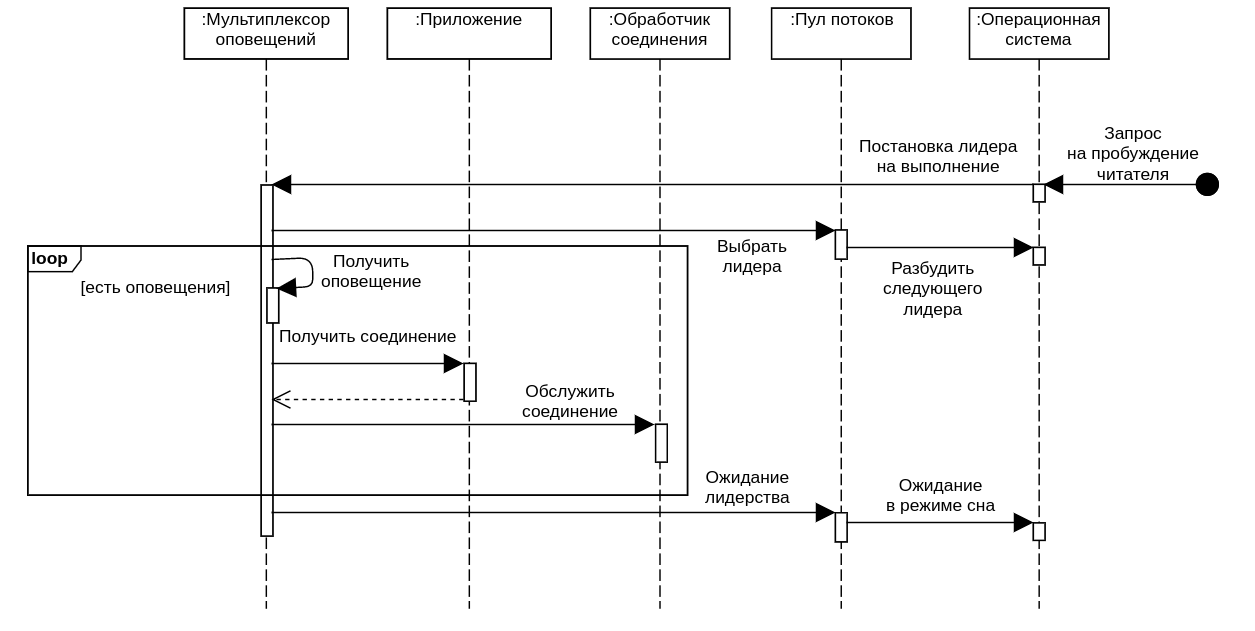
\includegraphics[width=\textwidth]{../../graphics/schemes/LFMuxSequence}
\end{figure}

В каждый момент времени состояние мультиплексора опрашивает не более одного потока, потока-лидера. При наличии оповещений для обслуживания, поток-лидер диспетчеризует в пул потоков постановку на выполнение нового лидера. Сам же он перестает быть лидером и занимается обслуживанием соединений, для которых получены оповещения. Это требует внесения изменений в процедуру опроса мультиплексора и обслуживания соединений. Изменения представлены на листинге \ref{appendix91:LFReceiverCode}. Среди них:
\begin{enumerate}
\item Поток-лидер должен запомнить все соединения, которые ему необходимо обслужить.
\item Каждое из этих соединений необходимо пометить как \textit{Handling}. Метод \textit{should\_process()} приведен на листинге \ref{chapter31:LFShouldProcess}.
\item Поток-лидер диспетчеризует нового лидера.
\item После обслуживания соединений для полученных оповещений поток переходит в состояние ожидания лидерства.
\end{enumerate}

\begin{lstlisting}[float=!h,caption={Процедура подготовления соединения к обслуживанию в модели обслуживания соединений ''Лидер/Последователи``},label={chapter31:LFShouldProcess},frame=tlrb]
bool IMultiplexerListener::should_process()
{
    std::unique_lock<std::mutex> lock(m_input_close_mutex);
    if (m_state == State::Closed) {
        return false;
    }
    if (m_state == State::Handling) {
        m_state = State::KeepHandling;
        return false;
    }
    m_state = State::Handling;
    return true;
}
\end{lstlisting}

Второй шаг необходим, так как в противном случае новый лидер может получить новое оповещение для уже обслуживаемых предыдущим лидером соединений и тогда два потока будут параллельно обслуживать одно и то же соединение, что недопустимо.

В настоящей работе реализована вариация метода, в которой поток-лидер обслуживает соединения для всех обнаруженных оповещений. Такой подход может быть эффективен, когда число одновременно активных соединений мало. Недостаток такой реализации состоит в худшем использовании параллелизма на уровне соединений и накоплении временной задержки на передачу данных в случае, если несколько соединений последовательно будут обслужены одним потоком. Как и в предыдущем методе, Поток-лидер может ожидать новых оповещений в состоянии сна на futex в случае их долгого отсутствия. В таком случае временная задержка на передачу данных также будет увеличена на время постановки потока мультиплексора на выполнение.

\subsubsection{Метод обслуживания соединений ''Лидер/Последователи`` с активным опросом мультиплексора}\label{chapter31:NonBlockingLF}

Как было сказано выше, время постановки на выполнение потока, опрашивающего мультиплексор, может влиять на временную задержку на передачу данных. Потому что для передачи данных необходимо сначала доставить процессу-читателю оповещение о том, что данные для него готовы.

Мультиплексор оповещений в разделяемой памяти состоит из двух уровней (см. рисунок \ref{chapter31:MuxZeroState}):
\begin{itemize}
\item 4-байтного числа futex, используемого для ожидания в режиме сна и пробуждения потока мультиплексора;
\item 32 8-байтных сигнальных чисел по одному на каждый бит числа на первом уровне.
\end{itemize}

Можно использовать иной метод ожидания оповещений -- активный опрос первого уровня мультиплексора вместо пребывания в режиме сна на futex. При таком подходе ядро ОС при оповещении процесса-читателя и для ожидания оповещений не задействуется.
Схема работы метода представлена на рисунке \ref{chapter31:MuxBusyWaitScheme}.

\begin{figure}[!h]
\caption{Диаграмма обслуживания соединений по методу ''Лидер/Последователи`` с активным опросом мультиплексора оповещений}
\label{chapter31:MuxBusyWaitScheme}
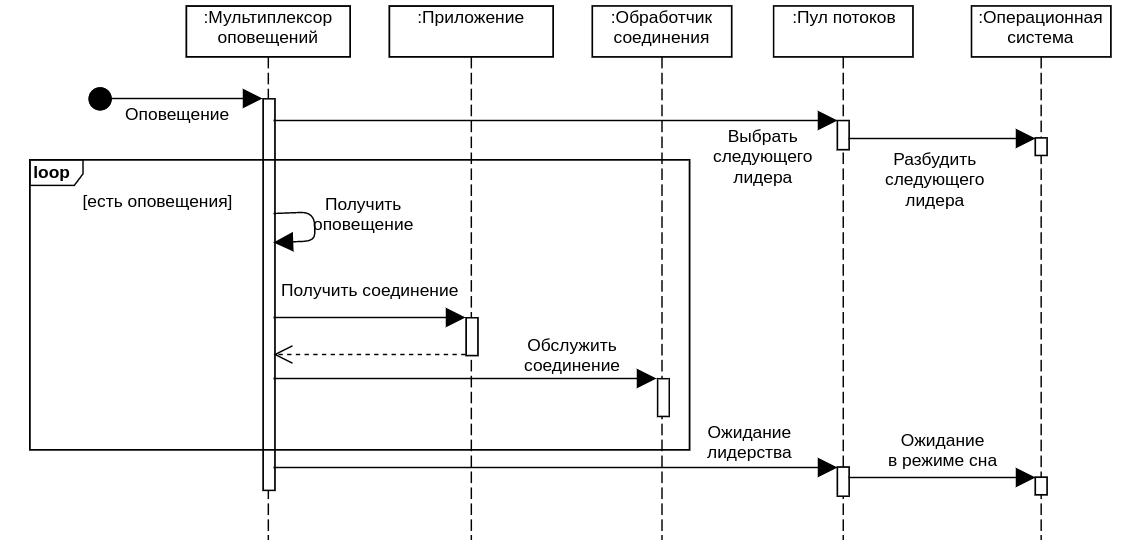
\includegraphics[width=\textwidth]{../../graphics/schemes/LFMuxSequenceSpin}
\end{figure}

Поток, опрашивающий мультиплексор, делает это без перерыва в рамках выделенного ему планировщиком ОС кванта процессорного времени. Такой подход называется холостым ожиданием (или же busy wait). Он используется в различных реализации циклических блокировок. Метод активного ожидания в применении к взаимным исключениям критикуется за пустую трату процессорного времени \cite{10.1007/3-540-44947-7_10, Ganjaliyev2019}. Но в применении к данной работе это допустимо, так как позволяет уменьшить временную задержку на передачу данных при соблюдении нескольких условий, связанных с планированием процессов в ОС:
\begin{itemize}
\item Достаточность аппаратных ресурсов. Каждый процесс, который будет использовать метод активного ожидания на мультиплексоре, будет постоянно занимать одно ядро процессора. В случае недостатка вычислительных мощностей планировщик задач может уменьшать доступное процессам процессорное время для сохранения качества обслуживания.
\item Время ожидания оповещений мало. В ростом времени активного опроса мультиплексора растет вероятность вытеснения потока мультиплексора с процессора. Поскольку поток мультиплексора ожидает оповещений только в пользовательском пространстве, ядру неизвестно, что поток надо будет поставить на выполнение при изменении состояния мультиплексора. Значит, временная задержка на передачу данных может значительно вырасти.
\end{itemize}

В методе обслуживания соединений ''Лидер/Последователи`` поток, который активно опрашивает мультиплексор, постоянно меняется. А значит, для потока-лидера уменьшаются шансы быть вытесненным с процессора по окончании кванта планирования. В отличие от него, в методе ''Полусинхронный/Полуреактивный`` только один поток занимался бы активным опросом мультиплексора, что приводило бы к его вытеснению с процессора из-за израсходования процессорного времени. Поэтому метод активного ожидания оповещений рассматривается только для метода обслуживания соединений ''Лидер/Последователи``.

Для реализации рассматриваемого метода необходимо изменить алгоритм работы двух процедур мультиплексора оповещений: процедуры оповещения и ожидания оповещений.

На листинге \ref{chapter31:BusyWait} приведена процедура ожидания оповещений. В отличие от методов с пассивным ожиданием оповещений, в рассматриваемом методе не используется системный вызов \textit{futex\_wait}. Поток-лидер циклически опрашивает первый уровень мультиплексора до тех пор, пока не будет получено оповещение. \textit{TBD: описать, зачем mm\_pause}

\begin{lstlisting}[float=!h,caption={Исходный код процедуры ожидания оповещений через мультиплексор событий в разделяемой памяти при использовании метода активного опроса мультиплексора},label={chapter31:BusyWait},frame=tlrb]
void Multiplexer::wait() {
	while (!m_futex) {
		_mm_pause();
	}
}
\end{lstlisting}

На листинге \ref{chapter31:BusyWake} приведена процедура ожидания оповещений. В отличие от методов с пассивным ожиданием оповещений, в рассматриваемом методе оповещение состоит исключительно в выставлении нужных битов в мультиплексоре. Системный вызов \textit{futex\_wake} также не нужен, так как процесс-читатель не находится в состоянии сна в ожидании оповещений.

\begin{algorithm}[!h]
\caption{Исходный код процедуры оповещения процесса через мультиплексор событий в разделяемой памяти при использовании метода активного опроса мультиплексора}
\label{chapter31:BusyWake}
\begin{lstlisting}[frame=tlrb]
void Multiplexer::notify(Signal id) {
	m_signal[id / Multiplexer::c_signals_per_chunk]
		.fetch_or(1 << id % Multiplexer::c_signals_per_chunk);
	uint32_t futex = m_futex
		.fetch_or(1 << id / Multiplexer::c_signals_per_chunk);
}
\end{lstlisting}
\end{algorithm}

Таким образом, удается избежать системных вызовов при передаче данных между процессами и временной задержки на постановку потока-лидера на выполнение. Чтобы обслужить соединения по полученным оповещениям, необходимо диспетчеризовать новый поток-лидер для обеспечения параллелизма на уровне соединений. Метод также обладает недостатками из-за метода холостого ожидания: \textbf{TBD: NB} непредсказуемыми задержками из-за планировщика процессов и неэффективным использованием процессорного времени.

\chapterconclusion

Разработан метод оповещения о появлении данных в очереди в разделяемой памяти посредством мультиплексора оповещений в разделяемой памяти. Мультиплексор оповещений позволяет отслеживать оповещения одновременно от 2048 соединений. Подавляющая часть работы с ним производится в пользовательском пространстве. Ядро ОС используется только для ожидания оповещений в режиме сна и для пробуждения процесса-читателя при оповещении. 
На его основе разработано семейство новых методов межпроцессного взаимодействия:
\begin{enumerate}
\item с пассивным ожиданием оповещений в мультиплексоре в режиме сна и обслуживанием соединений по методу ''Полусинхронный/Полуреактивный``.
\item С пассивным ожиданием оповещений в мультиплексоре в режиме сна и обслуживанием соединений по методу ''Лидер/Последователи``.
\item С активным опросом мультиплексора и обслуживанием соединений по методу ''Лидер/Последователи``.
\end{enumerate}

Рассмотрены их сильные и слабые стороны, даны рекомендации по их практическому применению. Сделаны предположения об их устройстве на влияние на временную задержку на передачу данных. \textbf{TBD: описать подробнее}
